%------------- ROBOT GENERAL DIMENSIONS -------------%
\subsection{Robot General Dimensions}

Figure \ref{fig:crab_dim} shows the general dimensional parameters of the robot. The center of origin is currently located in the geometric center of the chassis in $x$ and $y$ directions and at the bottom of the chassis in $z$. The crab consists of five legs named from A to E. The lengths of the thigh members and tibia members are identified with $L_{i}$ and $l_{i}$ respectively, where $i = A, B, C, D, or E$. Similarly, the angles of the thigh members are identified with $\theta_{i}$, whereas the angles of the tibia members are identified with $\phi_{i}$. Both of these angles are measured from the global positive x-axis in the xz-plane. Each node of the leg is identified by the letter of the leg (A to E) followed by an index of 1, 2 or 3 representing the hip, knee, and foot respectively.

\begin{figure}
    \centering
    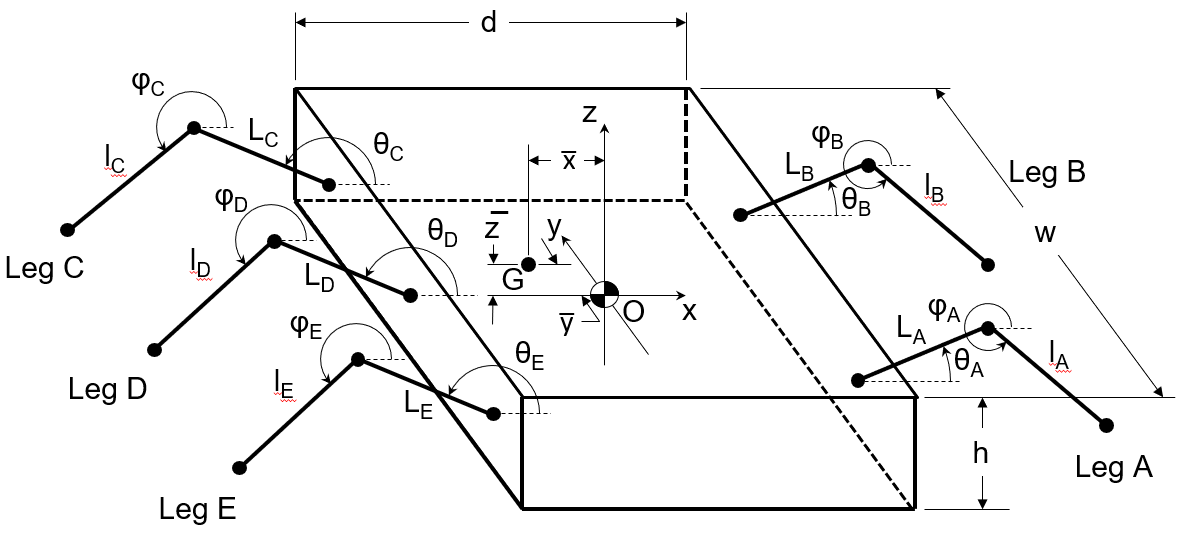
\includegraphics[width=\textwidth]{4_ComponentProperties/img/robot_dimensions.PNG}
    \caption{Crab General Dimensions}
    \label{fig:crab_dim}
\end{figure}

Table \ref{table:gen_dim} shows the values chosen for each parameter. The leg angles were chosen to represent the worst case of leg positioning for the robot. This is limited due to the fact that each joint will have a bellow cover, making the possible motion smaller. Chassis size was determined based on the component layout determined in the center of mass analysis.

\begin{table}[H]
\centering
  \caption{General Dimensions}
  \label{table:gen_dim}
  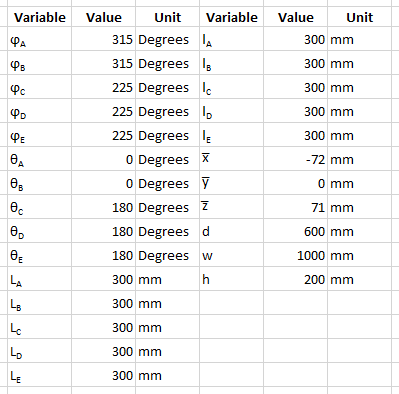
\includegraphics[width=0.5\textwidth]{4_ComponentProperties/img/GeneralDimensions.PNG}
\end{table}


%------------- BATTERY CODE DIMENSIONS -------------%
\subsection{Battery Requirements and Dimensions}

Cells are arranged into a battery and managed by a Battery Management System \cite{voltaplex_6s16s_nodate}. All electronics are powered from this with the necessary voltage regulators.
The battery voltage is defined as the highest voltage of any component, $V_{max}$, likely the motors running between 24 and 48 V.
The number of battery cells running in series, $N_{series}$, is defined as

\begin{equation}
    N_{series} = \frac{V_{max}}{V_{cell}} = \frac{V_{max}}{3.6 V}
\end{equation}

The number of cells in parallel, $N_{parallel}$, to achieve the desired run time is defined as

\begin{equation}
    N_{parallel} = \frac{T \cdot I}{Q} = \frac{[h] \cdot [A]}{[Ah]}
\end{equation}

where $T$ is the runtime in hours, $I$ is the total current draw of the robot and $Q$ is the Amp-hour rating of an individual battery cell \cite{digikey_electronics_battery_nodate}.

The total number of required cells is the number of series cells multiplied by the number of parallel cells.

\begin{equation}
    N = N_{parallel} \cdot N_{series}
\end{equation}

As an example, a tested configuration included a Maxon Motor EC90 260W and Maxon Motor EC60 200W per leg, Panasonic NCR18650B cells in the battery, as well as very conservative estimates for the power consumption of Group WR2Bs litter picker \cite{maxon_motor_ec60_nodate} \cite{harmonic_drive_csd-2a_nodate} \cite{panasonic_industrial_devices_specifications_nodate} \cite{18650batterystore_18650_nodate}.
The total current draw is 80 A, with a motor voltage of 48 V.
The number of cells in series is thus

\begin{equation}
    N_{series} = \frac{48 \text{V}}{3.6 \text{V}} = 13.33 \text{cells}
\end{equation}

This is rounded up the 14 cells in series.
The number of cells in parallel is calculated in the same way

\begin{equation}
    N_{parallel} = \frac{2 \text{hours} \cdot 80 \text{A}}{3.4 \text{Ah}} = 47.05 \text{cells}
\end{equation}

Again, this value is rounded up to 48 cells.
Finally, the total number of required cells in calculated

\begin{equation}
    N = 14 \cdot 48 = 672
\end{equation}

These cells could be split up into multiple batteries, or take different shapes and sizes.
An example script is found in Appendix \ref{app:battery} and gives one large battery that contains vertically aligned cells with as-close-to-square-as-possible width and length. In contrast, for the purpose of determining an approximate centre of mass, the cells were separated into four equal batteries in the center of mass calculation presented in
Section \ref{subsec:center_of_mass}.

%------------- CENTER OF MASS -------------%

\subsection{Centre of Mass} \label{subsec:center_of_mass}

The centre of mass was calculated with the following steps:
\begin{itemize}
    \item Assuming a total robot mass (namely assuming battery mass).
    \item Calculating required motor torques and selecting appropriate motors and harmonic drives.
    \item Calculating required battery size with motor and electronics power requirements.
    \item Making a layout of the components (legs, batteries, other groups' litter picker, etc.) within the chassis and determining their distance from the origin in the middle of the chassis.
    \item Calculating the centre of mass.
    \item Iterate.
\end{itemize}

The first iteration was done by assuming an equal normal force acting on all legs of the robot, as the centre of mass is ultimately required to get more precise normal forces (see equations for normal forces in Section \ref{sec:normal_forces}). These more precise normal forces were then used in the next iteration to get more extreme torques. 

The component layout was drafted based on the size and weight of the various components. Figure \ref{fig:component_layout} shows the general arrangement of components. The centre of mass of each component was assumed at its middle. The specific location coordinates were specified in an excel table (see Appendix \ref{app:centre_of_mass}), which took all components into consideration for the centre of mass calculation. The general chassis dimensions were also calculated as a consequence of this calculation.

\begin{figure}
    \centering
    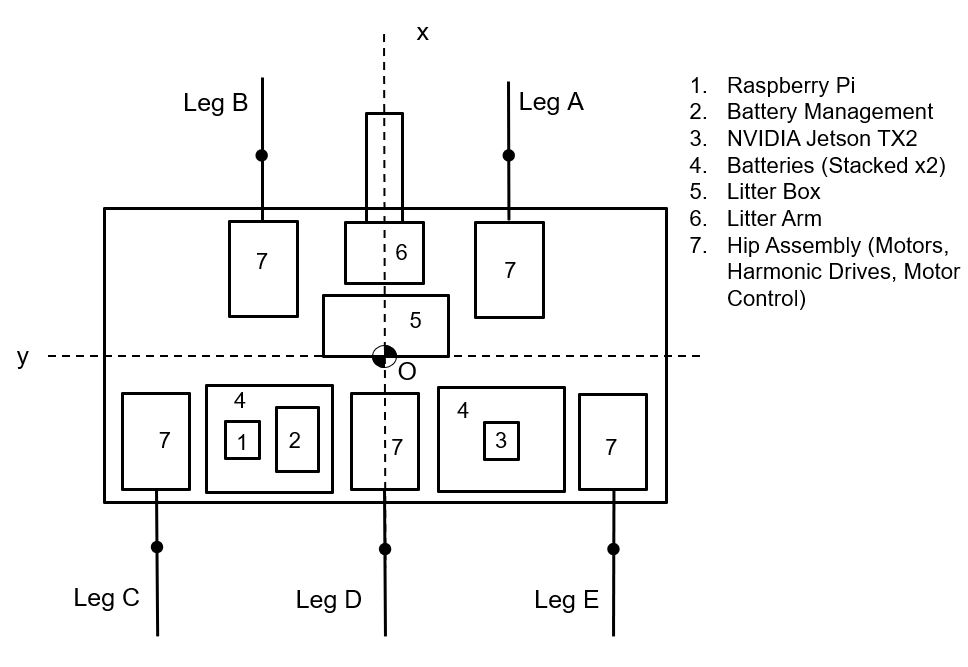
\includegraphics{4_ComponentProperties/img/component_layout.JPG}
    \caption{Layout of Components in Robot Chassis}
    \label{fig:component_layout}
\end{figure}

The centre of mass is given by the following equation. 

\begin{gather}
    x_{cm} = \frac{\sum m_i x_i}{\sum m_i}
    \hspace{2em}
    y_{cm} = \frac{\sum m_i y_i}{\sum m_i}
    \hspace{2em}
    z_{cm} = \frac{\sum m_i z_i}{\sum m_i}
\end{gather}

where $m_i$ are the mass of various components and $x_i$, $y_i$ and $z_i$ are the distance of the centre of mass of each component compared to the origin of the robot, on each axis. The centre of mass value is used to assess the stability of the robot in Section \ref{sec:stability}.